\section{Geometry and Functions}

Values of $x$ and $y$ can be represented by Cartesian coordinates $(x,y)$ on a graph.

\subsection{Equations of Lines and Circles}

\subsubsection{Equation of a Straight Line}

The general equation for a straight line between two variables $x$ and $y$ is 
\begin{align}
    \label{line-general} ax + by = p,
\end{align}
where $a$, $b$, and $p$ are constants. Equation \eqref{line-general} is commonly rearranged as 
\begin{align}
    \label{line} y = mx + c,
\end{align}
by defining the constants $m = -a/b$ and $c = p/b$. Note that equation \eqref{line} is less generic than equation \eqref{line-general} since it is not defined for the case of $b=0$.\\

\begin{definition}
 (gradient and $y$-intercept). The constant $m$ is the \textbf{gradient} of the straight line (\textit{i.e.} the relative change in $y$ for a given change in $x$). The constant $c$ is known as the \textbf{y-intercept} (\textit{i.e.} the value of $y$ at which the line crosses $x=0$).
\end{definition}

\begin{example}
(plotting a straight line). Given $m = 2$ and $c = 1$, plot the straight line given by equation \eqref{line} between $0 \leq x \leq 5$.
\end{example}
\begin{solution}
{
\begin{itemize}
\renewcommand{\labelitemi}{$\Rightarrow$}
\item We have $c=1$, therefore the line passes through $(0,1)$.
\item Substituting $x=5$ into equation \eqref{line} gives $y = 11$. Therefore, $(5,11)$ is another point on the line.
\end{itemize}
Figure \ref{fig:straight_line_pts} plots the resulting straight line.
}
\end{solution}

\begin{figure}[h!]
    \centering
    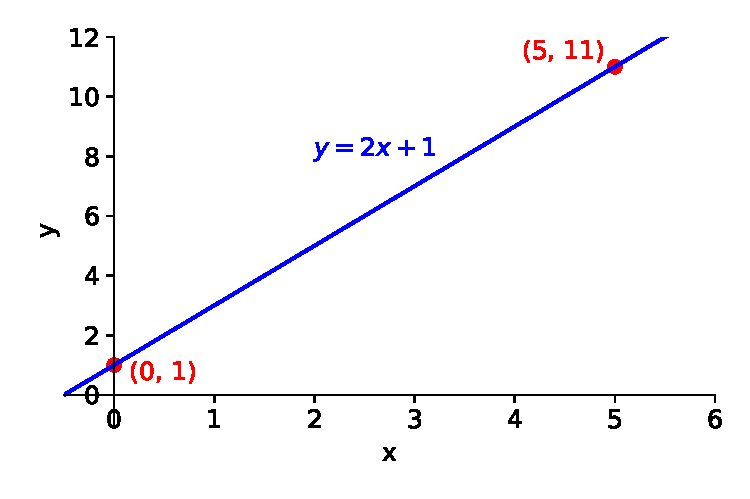
\includegraphics[width=0.5\textwidth]{Figures/example_111.pdf}
    \caption{Demonstration of plotting of $y=2x+1$ from Example 1.1.1.}
    \label{fig:straight_line_pts}
\end{figure}

Some useful properties of straight lines
\begin{itemize}
    \item Two lines are \textbf{parallel} if they have the same gradient.
    \item Two lines, with gradients $m_1$ and $m_2$, are \textbf{perpendicular} if $m_1 m_2 = -1$
    \item A \textbf{horizontal} line ($m = 0$) has equation $y = c$ 
    \item A \textbf{vertical} line ($b = 0$ in equation \eqref{line-general}) has equation $x = d$.
    \item Two straight lines cross where they have the same values of $x$ and $y$. 
\end{itemize}

\begin{example} 
Find the crossing point of the lines
\begin{align*}
    y &= x + 1 \\
    y &= -\frac{1}{2}x + 4. 
\end{align*}
\end{example} 
\fbox{
\begin{minipage}{0.95\textwidth}
We can find the crossing point $(x,y) = (\alpha, \beta)$ by solving the above equations simultaneously for $\alpha$ and $\beta$. Since the LHS is the same in both equations, we find
\begin{align*}
\alpha + 1 &= -\frac{1}{2} \alpha + 4 \\
\therefore \; \frac{3}{2} \alpha &= 3 \\
\therefore \; \alpha &= 2.
\end{align*}
Now, substituting this into \textit{e.g.} $y = x + 1$ for $x$, we get $b = 3$ and hence the crossing point is at $(x,y) = (2,3)$.
\end{minipage}}\\

\begin{definition}
\label{def:Edist}
    (Euclidean distance between two points). The \textbf{Euclidean distance} (\textit{i.e. straight line distance} between two points $(x_1, y_1)$ and $(x_2, y_2)$ in Cartesian coordinates is $d = \sqrt{(x_2-x_1)^2 + (y_2-y_1)^2}$. %This can be shown using Pythagoras rule (see figure \ref{fig:distance})/ 
\end{definition}

\subsubsection{Equation of a Circle}

The equation for a circle in Cartesian coordinates $(x,y)$ with centre at $(a,b)$ and radius $R$ is given by
\begin{align}
    \label{circle} (x - a)^2 + (y-b)^2 = R^2.
\end{align}
Using Definition \ref{def:Edist} we can see that the radius $R$ is the straight line distance between the points on the circle and its centre (which makes sense!).\\ %(see figure \ref{fig:distance})/ 

\begin{example}
    Find the centre and radius of the circle with equation
    \begin{align*}
        x^2 + 4x + y^2 - 6y = 3
    \end{align*}
\end{example}
\fbox{
\begin{minipage}{0.95\textwidth}
If we expand the equation of a circle (equation \eqref{circle}) and move the constant terms to the RHS, we find
\begin{align*}
    x^2 - 2ax + y^2 - 2by = R^2 - a^2 - b^2. \\ 
\end{align*}
Comparing the coefficients of $x$ and $y$ with the terms in the expression in the example, we see $-2a=4$ and $-2b=-6$, therefore $a=-2$ and $b=3$. Now comparing the RHS of both equations we see that $R^2-a^2-b^2=3$, which means $R^2 = 16$. Therefore, the centre of the circle is at $(x,y) = (-2,3)$ and its radius is $R=4$. 
\end{minipage}}\\

\begin{definition}
    (crossing points between a line and circle). To find the crossing points between two curves, the equations for the two curves need to be solved simultaneously. To do this, we can substitute the equation for the line (equation \eqref{line}) into the equation for the circle (equation \eqref{circle}). This leads to a quadratic equation in $x$ that can yield
    \begin{itemize}
        \item Two unique real solutions for $x$, meaning two crossing points.
        \item One (repeated) solution, meaning there is one crossing point and the line is tangent to the circle.
        \item No real solutions, meaning the line and circle do not cross.
    \end{itemize}
    %These outcomes are illustrated in figure \ref{fig:line_and_circle}.
\end{definition}

\begin{example} 
Do the following line and circle cross, if so, at what point(s)?
\begin{align*}
    y &= x + 1 \\
    (x - 1)^2 + (y-2)^2 &= 8
\end{align*}
\end{example} 
\fbox{
\begin{minipage}{0.95\textwidth}
Substituting the first equation into the second (for $y$) gives
\begin{align*}
    (x-1)^2 + (x+1-2)^2 &= 8\\
    \therefore 2(x-1)^2 &= 8\\
    \therefore x-1 &= \pm 2\\
    \therefore x &= \{-1,\; 3\}
\end{align*}
The corresponding $y$ values can be acquired easily by substituting into the equation for the line $y = x + 1$, which means there are two crossing points at $(-1,0)$ and $(3,4)$.
\end{minipage}}\\

\begin{definition}
    (lines tangent and normal to a circle). A line that passes through a point $P$ on the circle and its centre (\emph{i.e.} along the radius) is \textbf{normal} to the circle at that point. The \textbf{tangent} line is perpendicular to the normal (and therefore parallel to the circle) at the point $P$.
\end{definition}

\begin{definition}
    (perpendicular bisector of a chord). A line that passes through two points $A$ and $B$ on the circle is called a \textbf{chord}. The perpendicular bisector of this (\emph{i.e.} the line that is perpendicular to the line $AB$ and crosses it at its midpoint) will pass through the centre of the circle. %These outcomes are illustrated in figure \ref{fig:line_and_circle}.
\end{definition}

\begin{example}
    Find the equation of a circle with centre along the line $y=2x-3$ and which also passes through the two points (1,6) and (5,2). 
\end{example}
\fbox{
\begin{minipage}{0.95\textwidth}
The chord between points $A(1,6)$ and $B(5,2)$ has gradient $m = (2-6)/(5-1) = -1$. Therefore, the line perpendicular to this chord will have gradient $1$ and so equation $y = x + c$. The centre of the chord is at the point $(A+B)/2 = (3,4)$, therefore substituting $x=3$ and $y=4$ into $y = x + c$ gives $c = 1$, and so $y=x+1$ is a perpendicular bisector of the chord and so pass through the centre of the circle. 

We know that $y=2x-3$ also passes through the centre, so the point where $y=2x-3$ and $y=x+1$ cross must be the centre. Equating the RHS of each gives $2x-3=x+1$ and so $x=4$, and therefore $y=5$. Therefore, the equation will be of the form $(x-4)^2 + (y-5)^2 = R^2$. To find $R$, we can substitute in any point on the circle (as they all must satisfy this equation). Substituting in $A$ we find $(1-4)^2+(6-5)^2=R^2$ and so $R^2=10$. So, finally, the equation of the circle is given by
\begin{align*}
    (x-4)^2 + (y-5)^2 = 10.
\end{align*}
We can check this solution by substituting in the point $B$ and noting that it also satisfies the equation. 
\end{minipage}}

\newpage
\subsection{Parametric and Implicit Functions}

When discussing functions so far we have usually focused on the \textbf{explicit} form $y = f(x)$ which directly relates the value of $x$ to the corresponding value of $y$. In this section we will look at alternative ways to represent the relationships between the variables $x$ and $y$.

\subsubsection{Parametric Functions}

A parametric function introduces a \textbf{parameter} (\textit{e.g.} $t$) and expresses our variables in terms of this parameter, such that 
\begin{align}
    x = g(t) \quad \mathrm{and} \quad y = h(t). 
\end{align}
Parametric functions arise naturally in many contexts (\textit{e.g.} when measuring how two quantities $x$ and $y$ change with time $t$). They are also useful in many circumstances as a way to simplify the relationship between $x$ and $y$.\\

Note, however, that not all parametric functions can be expressed in explicit form $y = f(x)$ and often the parametric form of $x$ and $y$ means they may be restricted to certain value ranges. In general, if the equation for $x$ can be rearranged to give $t$ as a function of $x$, this can be substituted into the equation for $y$ to give the explicit form. However, this is not necessarily always the best way to find the explicit form.\\

\begin{example}
    Sodium oxide (Na$_2$O) is placed in water, each molecule of Na$_2$O reacts with H$_2$O to produce 2 molecules of sodium hydroxide (NaOH). The number of molecules of Na$_2$O and NaOH in solution with respect to time $t \geq 0$ is given by $x = x_0e^{-\alpha t}$ and $y = 2x_0(1 - e^{-\alpha t})$ respectively, where the constant $x_0$ is the initial number of molecules of Na$_2$O. Write the number of sodium hydroxide molecules $y$ as a function of the number of sodium oxide molecules $x$, noting any restrictions on $x$ and $y$. 
\end{example}
\fbox{
\begin{minipage}{0.95\textwidth}
The parametric form of $x$ can be rearranged as $\exp(-\alpha t) = x/A$ and we can substitute this into the equation for $y$ to see that $y = 2(x_0-x)$. Since $t \geq 0$, $x$, is restricted to be between $x_0$ (at $t=0$) and $0$ (as $t \rightarrow \infty$). Similarly, $y$ is restricted to be between $0$ (at $t=0$) and $2x_0$ (as $t \rightarrow \infty$). Therefore we can write $0 \leq x \leq x_0$ and $0 \leq y \leq 2x_0$.\\

We see this makes sense with the description of the reaction. At $t=0$, $x = x_0$ and so $y = 0$, as the reaction proceeds, for every molecule of $x$ that is lost, $y$ increases by 2, until eventually converging towards $x \rightarrow 0$ and $y \rightarrow 2x_0$. 
\end{minipage}}\\

\begin{example}
\label{eg:parametric_circle}
     Express the circle with centre at (2,3) and radius 4 in parametric form.
\end{example}
\fbox{
\begin{minipage}{0.95\textwidth}
The standard way to represent a circle in parametric form is to use the angle $0 \leq \theta < 2\pi$ that radius of the circle makes with the $x$-direction. All points on the circle are the same distance $R$ from the centre $(a,b)$, so we can write $x=a+R\cos\theta$ and $y=b+R\sin \theta$. Substituting in the values gives the parametric form for this case 
\begin{align*}
    x&=2+4\cos\theta\\
    y&=3+4\sin\theta.
\end{align*}
We can check this by substituting into the non-parametric form $(x-2)^2+(y-3)^2=16$. and seeing that it satisfies the equation.
\end{minipage}}\\

\subsubsection{Implicit Functions}

Implicit functions are those written in the form $g(x,y) = 0$, as opposed to explicit functions of the form $y = f(x)$. In many cases, this form is more general (\textit{e.g.} there might be multiple solutions for $y$ and expressing as $y = f(x)$ may suppose only one of them). Note, we have already seen the implicit form for a straight line in equation \eqref{line-general} and for a circle in equation \eqref{circle}.
\begin{example}
    \label{eg:ellipse} An ellipse can be written in implicit form as
    \begin{align*}
        \frac{x^2}{100} + \frac{y^2}{25} = 1.
    \end{align*}
    For $x = -10, -8, -6, 0, 6, 8, 10$ find possible values of $y$ and hence draw the ellipse.
\end{example}
\fbox{
\begin{minipage}{0.95\textwidth}
Rearranging into explicit form $y = \pm 5\sqrt{1 - x^2/100}$. Note that this is the same for $\pm x$ so substituting in $x = \pm10, \pm8, \pm6, 0$ we get $y = 0, \pm3, \pm4, \pm 5$ respectively. These points are plotted in figure \ref{fig:ellipse} along with the outline of the ellipse. 
\end{minipage}}\\

\begin{figure}[h!]
    \centering
    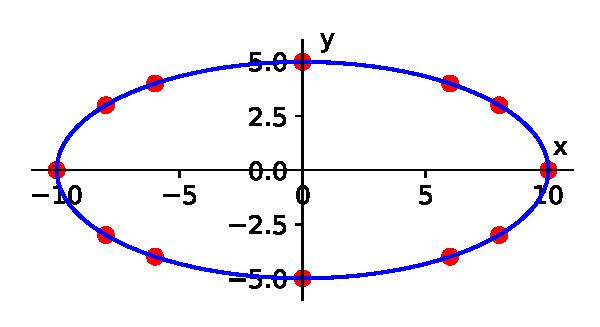
\includegraphics[width=0.5\linewidth]{Figures/example_123.pdf}
    \caption{Plot of the ellipse and calculated points in example \ref{eg:ellipse}.}
    \label{fig:ellipse}
\end{figure}


\newpage
\subsection{Partial Fraction Decomposition}

\subsubsection{Partial fractions in general}

``Partial fractions'' is a term used to describe the separation of a rational fraction (where both the numerator and denominator are both polynomials) into a sum of simplified rational fractions each with an irreducible polynomial on the denominator. It is often preferable to decompose a rational fraction into partial fractions for the purposes of differentiation or integration (which we will cover in section \ref{sec:calculus}).\\

The reverse procedure (expressing partial fractions as a single rational fraction) is much easier to achieve, as shown in the following example.

\begin{example}
    Express $1/(x+1) + 3/(x-2)$ as a single rational fraction.
\end{example}
\fbox{
\begin{minipage}{0.95\textwidth}
Multiplying the numerator and denominator of a fraction by the same expression does not change its value (except at troublesome points where the expression is 0, which we will ignore for now). So, we multiply numerator and denominator of each fraction by the denominator of the other, to get 
\begin{align*}
    &\frac{1}{x+1} + \frac{3}{x-2}\\
    &=\frac{x-2}{(x+1)(x-2)} + \frac{3(x+1)}{(x+1)(x-2)}\\
    &= \frac{4x-1}{(x+1)(x-2)}.
\end{align*}
\end{minipage}}\\

An example of partial fraction decomposition then would be to begin with $\frac{4x-1}{(x+1)(x-2)}$ and simplify it to $\frac{1}{x+1} + \frac{3}{x-2}$. Clearly, this is less straight-forward and so we need some generic rules that we can apply to solve this type of problem.\\

The process for decomposing into partial fractions depends on whether the fraction is proper or improper and whether the polynomials can be factorised.   

\begin{definition}
    (proper and improper rational fractions) A rational fraction is defined as \textbf{proper} if $d > n$ where $d$ is the degree of the polynomial in the denominator and $n$ is the degree of the polynomial in the numerator. It is improper if $n \geq d$. 
\end{definition}

\begin{example}
    Determine whether $(ax + b)^2/(cx^2 + d)$ is a proper rational fraction, where $a$, $b$, $c$, and $d$ are constants and $x$ is the independent variable.
\end{example}
\fbox{
\begin{minipage}{0.95\textwidth}
The numerator $(ax + b)^2$ is a polynomial of degree 2 (as the largest power of $x$ in the numerator is $x^2$) and the denominator $(cx^2 + d)$ is also degree 2. Therefore $d = n$ and so the fraction is improper.\\
\end{minipage}}\\

The steps for decomposing a rational fraction $f(x)/g(x)$ into partial fractions are as follows
\begin{enumerate}
    \item Factorise the polynomial denominator $g(x) = g_1(x)g_2(x)\ldots$
    \item Use this factorisation to write the functional form of the partial fractions $f_0(x) + f_1(x)/g_1(x) + f_2(x)/g_2(x) + \ldots$ using the rules in definitions \ref{def:linear_pf} -- \ref{def:improper}. 
    \item Equate both sides $f(x)/g(x) = f_0(x) + f_1(x)/g_1(x) + f_2(x)/g_2(x) + \ldots$, solve for the unknown coefficients in $f_1(x)$, $f_2(x)$, $\ldots$ by multiplying through by $g(x)$ to get a polynomial on both sides and comparing coefficients.
\end{enumerate}
This will make more sense with examples, which we can attempt once we have introduced some of the rules needed to complete step 2.

\subsubsection{Decomposition of proper fractions}
\label{sec:proper_fracs}

\begin{definition}
\label{def:linear_pf}
    (Partial fraction decomposition for proper fractions with linear factors in the denominator). If the fraction is proper and its denominator factorises into linear expressions in $x$ (\textit{i.e.} $g(x) = (x-a)(x-b)\ldots$ we can write
    \begin{align}
        \label{linear_pf} \frac{f(x)}{(x-a)(x-b)\ldots} = \frac{A}{x-a} + \frac{B}{x-b} + \ldots ,
    \end{align}
    where $A$ and $B$ are constant coefficients to be determined. 
\end{definition}

\begin{example}
    Express $(x-4)/(2x^2+5x-3)$ as partial fractions.
\end{example}
\fbox{
\begin{minipage}{0.95\textwidth}
First, we factorise the denominator to get $(x - 4)/[(x+3)(2x-1)]$, then use the rule in equation \eqref{linear_pf} to write
\begin{align*}
    \frac{x - 4}{(x+3)(2x-1)} &= \frac{A}{x+3} + \frac{B}{2x-1},\\
    \therefore x-4 &= A(2x-1) + B(x+3)
\end{align*}
Rather than comparing coefficients, in the case of two linear factors it is easier to evaluate the above at $x=-3$ and $x=1/2$ to yield $A = 1$ and $B = -1$ directly, and so
\begin{align*}
    \frac{x-4}{2x^2+5x-3} = \frac{1}{x+3} - \frac{1}{2x-1}.
\end{align*}
\end{minipage}}\\

\begin{example}
    Express $(2x^2+8x+18)/[x(x+2)(x-3)]$ as partial fractions.
\end{example}
\fbox{
\begin{minipage}{0.95\textwidth}
The denominator is already factorised into linear factors and the fraction is proper so we can use equation \eqref{linear_pf} to write
\begin{align*}
    \frac{2x^2+8x+18}{x(x+2)(x-3)} &= \frac{A}{x} + \frac{B}{x+2} + \frac{C}{x-3},\\
    \therefore 2x^2+8x+18 &= A(x+2)(x-3) + Bx(x-3) + Cx(x+2) \\
    \therefore 2x^2+8x+18 &= (A + B + C)x^2 + (-A -3B +2C) - 6A.
\end{align*}
Comparing the constant coefficients first we see $-6A=181$ and so $A=-3$. Comparing coefficients of the $x^2$ and $x$ terms then leaves
\begin{align*}
B + C &= 5\\
-3B+2C &= 5,
\end{align*}
which yields $C = 4$ and $B=1$. Therefore
\begin{align*}
    \frac{2x^2+8x+18}{x(x+2)(x-3)} &= -\frac{3}{x} + \frac{1}{x+2} + \frac{4}{x-3}.
\end{align*}
\end{minipage}}\\

\begin{definition}
    (Partial fraction decomposition for proper fractions with repeated linear factors in the denominator). If the fraction is proper and its denominator contains a linear fractor that is repeated (\textit{i.e.} $g(x) = (x-a)^2\ldots$ we can write
    \begin{align}
        \label{linear_repeat_pf} \frac{f(x)}{(x-a)^2\ldots} = \frac{A}{x-a} + \frac{B}{(x-a)^2} + \ldots,
    \end{align}
    where $A,B$ are constant coefficients to be determined. 
\end{definition}

\begin{example}
    Decompose $(2x - 5)/(x^2-6x+9)$ into partial fractions.
\end{example}
\fbox{
\begin{minipage}{0.95\textwidth}
First, factorise the denominator and then use the rule in equation \eqref{linear_repeat_pf} to write
\begin{align*}
    \frac{2x-5}{(x-3)^2} &= \frac{A}{x-3}+\frac{B}{(x-3)^2}\\
    \therefore 2x - 2 &= A(x-3) + B\\
    \therefore 2x - 2 &= Ax + (B - 3A)
\end{align*}
and so comparing coefficients gives $A = 2$ and $B-3A=-5$, therefore $B=1$, and so 
\begin{align}
    \frac{2x - 5}{x^2-6x+9} = \frac{2}{x-3} + \frac{1}{(x-3)^2}.
\end{align}
\end{minipage}}\\

\begin{definition}
    (Partial fraction decomposition for proper fractions with quadratic factors in the denominator). If the fraction is proper and one of the factors of the denominator is an irreducible quadratic in $x$ (\textit{i.e.} $g(x) = (ax^2+bx+c)\ldots$ then
    \begin{align}
        \label{quadratic_pf} \frac{f(x)}{(ax^2+bx+c)\ldots} = \frac{Ax+B}{ax^2+bx+c} + \ldots,
    \end{align}
    where $A,B$ are constant coefficients to be determined. 
\end{definition}

\begin{example}
    Express $x^2/(x-1)(x^2+3x-3)$ as a partial fraction.
\end{example}
\fbox{
\begin{minipage}{0.95\textwidth}
We see that $x^2+3x-3$ cannot be factorised and so the denominator cannot be factorised further and so we use the rule in equation \eqref{quadratic_pf} to write
\begin{align*}
    \frac{x^2}{(x-1)(x^2+3x-3)} &= \frac{A}{x-1} + \frac{Bx+C}{x^2+3x-3}\\
    \therefore x^2 &= A(x^2+3x-3) + (Bx+C)(x-1)\\
    \therefore x^2 &= (A+B)x^2 + (3A+B+C)x - (C+3A)
\end{align*}
Comparing coefficients we see that $C=-3A$, and so $B=0$. Therefore $A=1$ and $C=-3$, giving  
\begin{align*}
    \frac{x^2}{(x-1)(x^2+3x-3)} = \frac{1}{x-1} - \frac{3}{x^2+3x-3}.
\end{align*}
\end{minipage}}\\

\subsubsection{Decomposition of improper fractions}

\begin{definition}
\label{def:improper}
    (partial fraction decomposition of improper fractions). For improper fractions, where $n > d$, we need to account for the extra orders of the polynomial in the numerator by adding a polynomial to the RHS of order $n-d$, i.e.
    \begin{align}
        \label{improper} \frac{f(x)}{g(x)} = a_0 + a_1x + \ldots a_{n-d} x^{n-d} + \ldots
    \end{align}
    where the constants $a_0, \ldots, a_{n-d}$ are to be determined. what follows this polynomial on the RHS depends on the form of $g(x)$, using the same rules as for proper fractions in section \ref{sec:proper_fracs}.
\end{definition}

\begin{example}
    Express $3(x+1)^2/(x^2+x-2)$ as partial fractions.
\end{example}
\fbox{
\begin{minipage}{0.95\textwidth}
First we factorise the denominator to $(x - 1)(x + 2)$. The numerator and denominator have the same order, so the fraction is improper with $n-d=0$. Using the rules in \eqref{improper} and \eqref{linear_pf} we can write
\begin{align*}
    \frac{3(x+1)^2}{(x - 1)(x + 2)} &= A + \frac{B}{x-1} + \frac{C}{x+2}\\
    \therefore 3x^2 + 6x + 3 &= A(x^2 + x -2) + B(x+2) + C(x-1) \\
    \therefore 3x^2 + 6x + 3 &= Ax^2 + (A+B+C)x + (-2A+2B-C).
\end{align*}
Comparing $x^2$ coefficients we find $A = 3$, and so comparing the $x^1$ and $x^0$ coefficients we have $B+C=3$ and $2B-C=9$. This gives $C = -1$ and $B = 4$ and so
\begin{align*}
    \frac{3(x+1)^2}{x^2+x-2} = 3 + \frac{4}{x-1} - \frac{1}{x+2}
\end{align*}
\end{minipage}}\\

\begin{example}
    Write the partial fractions form of the following
    \begin{align*}
        \frac{5x^6 - 50x^5 + 386x^4 - 1074x^3 + 644x^2 + 1174x - 1354}{(x-2)^2(x^2-6x+50)},
    \end{align*}
    but do not find the values of the coefficients.
\end{example}
\fbox{
\begin{minipage}{0.95\textwidth}
The polynomial in the numerator is order 6, while the denominator is order 4, so from definition \ref{def:improper} we know the RHS must contain a quadratic. In the denominator, the first linear terms are repeated, so we use the rule in equation \ref{linear_repeat_pf}, and he quadratic expression cannot be factorised so we use the rule in equation \ref{quadratic_pf}. Putting all this together we see that the partial fraction decomposition must have the following form
\begin{align*}
    Ax^2 + Bx + C + \frac{D}{x-2} + \frac{E}{(x-2)^2} + \frac{Fx+G}{x^2-6x+50}.
\end{align*}
\end{minipage}}


